\documentclass[11pt]{article}
\usepackage{acl2015}
\usepackage{times}
\usepackage{svg}
\usepackage{url}
\usepackage{latexsym}
\usepackage{graphicx}
\usepackage{hyperref}
\usepackage[font={small}]{caption}

%\setlength\titlebox{5cm}

% You can expand the titlebox if you need extra space
% to show all the authors. Please do not make the titlebox
% smaller than 5cm (the original size); we will check this
% in the camera-ready version and ask you to change it back.


\title{Scattertext: a Browser-Based Tool for Visualizing how Corpora Differ}

\author{Jason S. Kessler \\
  CDK Global \\
  {\tt jason.kessler@gmail.com}  \\}

\date{}

\begin{document}
\maketitle
\begin{abstract}
  To do
\end{abstract}

\section{Introduction}
Finding words and phrases that discriminate categories of text is a common application of statistical NLP. For example, finding words that are most strongly characteristic of a political party in congressional speeches can help political scientist identify means of partisan framing \cite{monroe08,grimmer2010}, identifying differences in word usage between male and female characters in films can highlight narrative archetypes. \cite{schofield2016gender}, and language use in social media can inform personality types \cite{Schwartz13}.  Beyond these applications in social science, the identification of characteristic terms is also useful in 

While these studies all identify and rank category-discriminating words, a broad range of visualization techniques are used.  These include ranked lists of words, word clouds, word bubbles, and scatter clouds of words.  In Section \ref{related}, I will examine the objectives, strengths and weaknesses of these visualization techniques.

The interactive visualization package Scattertext\footnote{\href{http://www.github.com/JasonKessler/scattertext}{github.com/JasonKessler/scattertext}} will be introduced in Section \ref{scattertext}, its features motivated by the critiques in Section \ref{related}.  Special attention is paid to visualizing the output of sparse log-linear classifiers (e.g., l1-penalized logistic regression or ElasticNet).  

A related visualization task is identifying discriminating words that are semantically similar to a query.  For example, generating a visualizing that shows how members of opposing political parties use words that are similar to ``jobs'' or ``medicine'' differently. Scattertext's approach to this task--based in vector representations--is described in Section \ref{embeddings}.  

\section{Text Visualizations}
\label{related}
The simplest visualization, a list of words ranked by their scores is easy to produce, interpret and is thus ubiquitous.  There are numerous ways of producing word scores for ranking which are throughly covered in previous work.  The reader is directed to Monroe et al. \shortcite{monroe08} for an overview of model-based term scoring algorithms.  Also of interest, Bitvai and Cohn \shortcite{Bitvai15} present a method for finding sparse words and phrase scores from a trained ANN (with bag-of-words features) and its training data. 

Regardless of how complex the calculation word scores capture a number of different measures of word-association, which can be interesting when viewed independently, instead of as part of a unitary score.  These include: 

\begin{itemize}  
\item \textbf{Precision}. A word's discriminative power regardless of its frequency, or $P(\mbox{class}|\mbox{word}).$  A term that appears once in the categorized corpus will have perfect precision.
\item \textbf{Recall}. The frequency a word appears in a particular class, or $P(\mbox{word}|\mbox{class})$.  The variance of precision tends to decrease as recall increases.  Extremely high recall words tend to be stop-words. 
\item \textbf{Non-redundancy}. The level of a word's discriminative power given other words that co-occur with it.  If a word $w_a$ always co-occurs with $w_b$ and word $w_b$ has a higher precision and recall, $w_a$ would have a high level of redundancy. Measuring redundancy is non-trivial, and has traditionally been approached through l1, l2, or ElasticNet penalized logistic regression \cite{joshi2010}, as well as through other feature selection techniques.  
\item \textbf{Characteristicness}. How frequently the term appears in the corpus being studied relative to larger background corpus.  For example, if the categories of documents being compared are Tweets about two baseball teams and the background corpus is a sample of all of Twitter, than words like ``playoff'' or ``\#baseball'' would be characteristic of the general corpus, since they discriminate the corpus in general but not necessarily one category \cite{vennclouds}.
\end{itemize}

Complex text visualizations (i.e., not word lists) manipulate the position and appearance of words or points representing them to indicate their relative scores in these measures. For example, in Schwartz et al. \shortcite{Schwartz13}, two word clouds are given, one per each category of text being compared.  Words are sized by their linear regression coefficients (a composite metric of precision, recall and redundancy) and colored based on how frequently words occurred-- a metric closely associated with recall.  Words selected to include in clouds have minimum frequency threshold, 

(2) bubbles (cite bostock (nytimes)) y-axis, limited space, interactive

(3) log-odds with prior \cite{monroe08}.  disadvantage: includes a lot of empty space.  Only the about the top 10 terms can be labeled.

(4) scatter plots (rudder, tidytext).  Mention that important points tend to occur in the upper left and lower-right hand corners, and the hull.  

\subsection{Problems with existing scatter plots}

Many authors have followed \cite{monroe08} 

Words stack atop each other, as seen in (previous fig).  This generally renders all but the most prominent words unreadable. Past solutions to this problem have been externally labeling points \cite{schofield2016gender} and 

\begin{figure}[h]
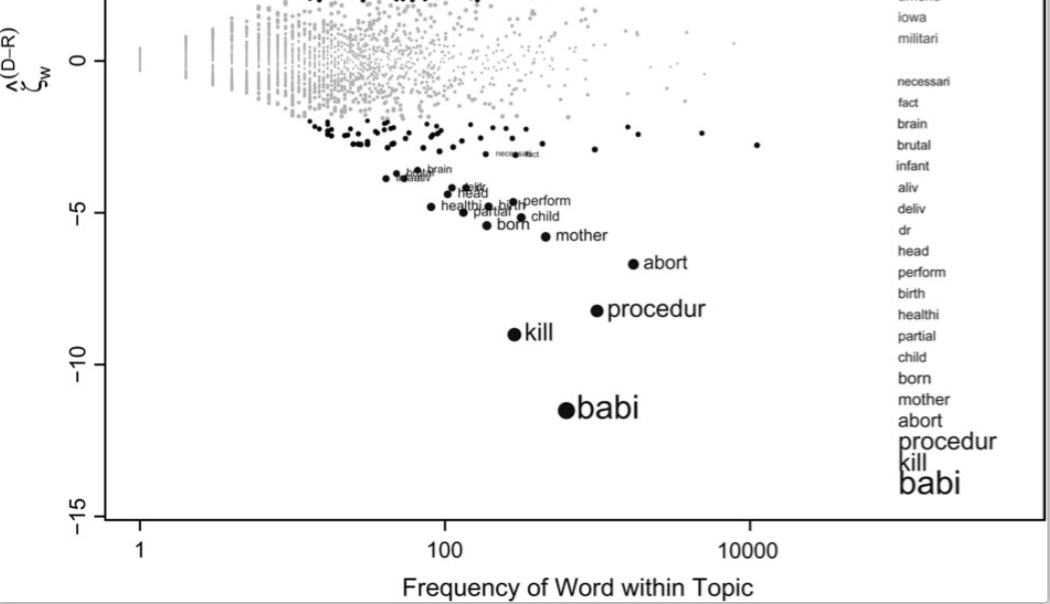
\includegraphics[width=\columnwidth]{monroehalf}
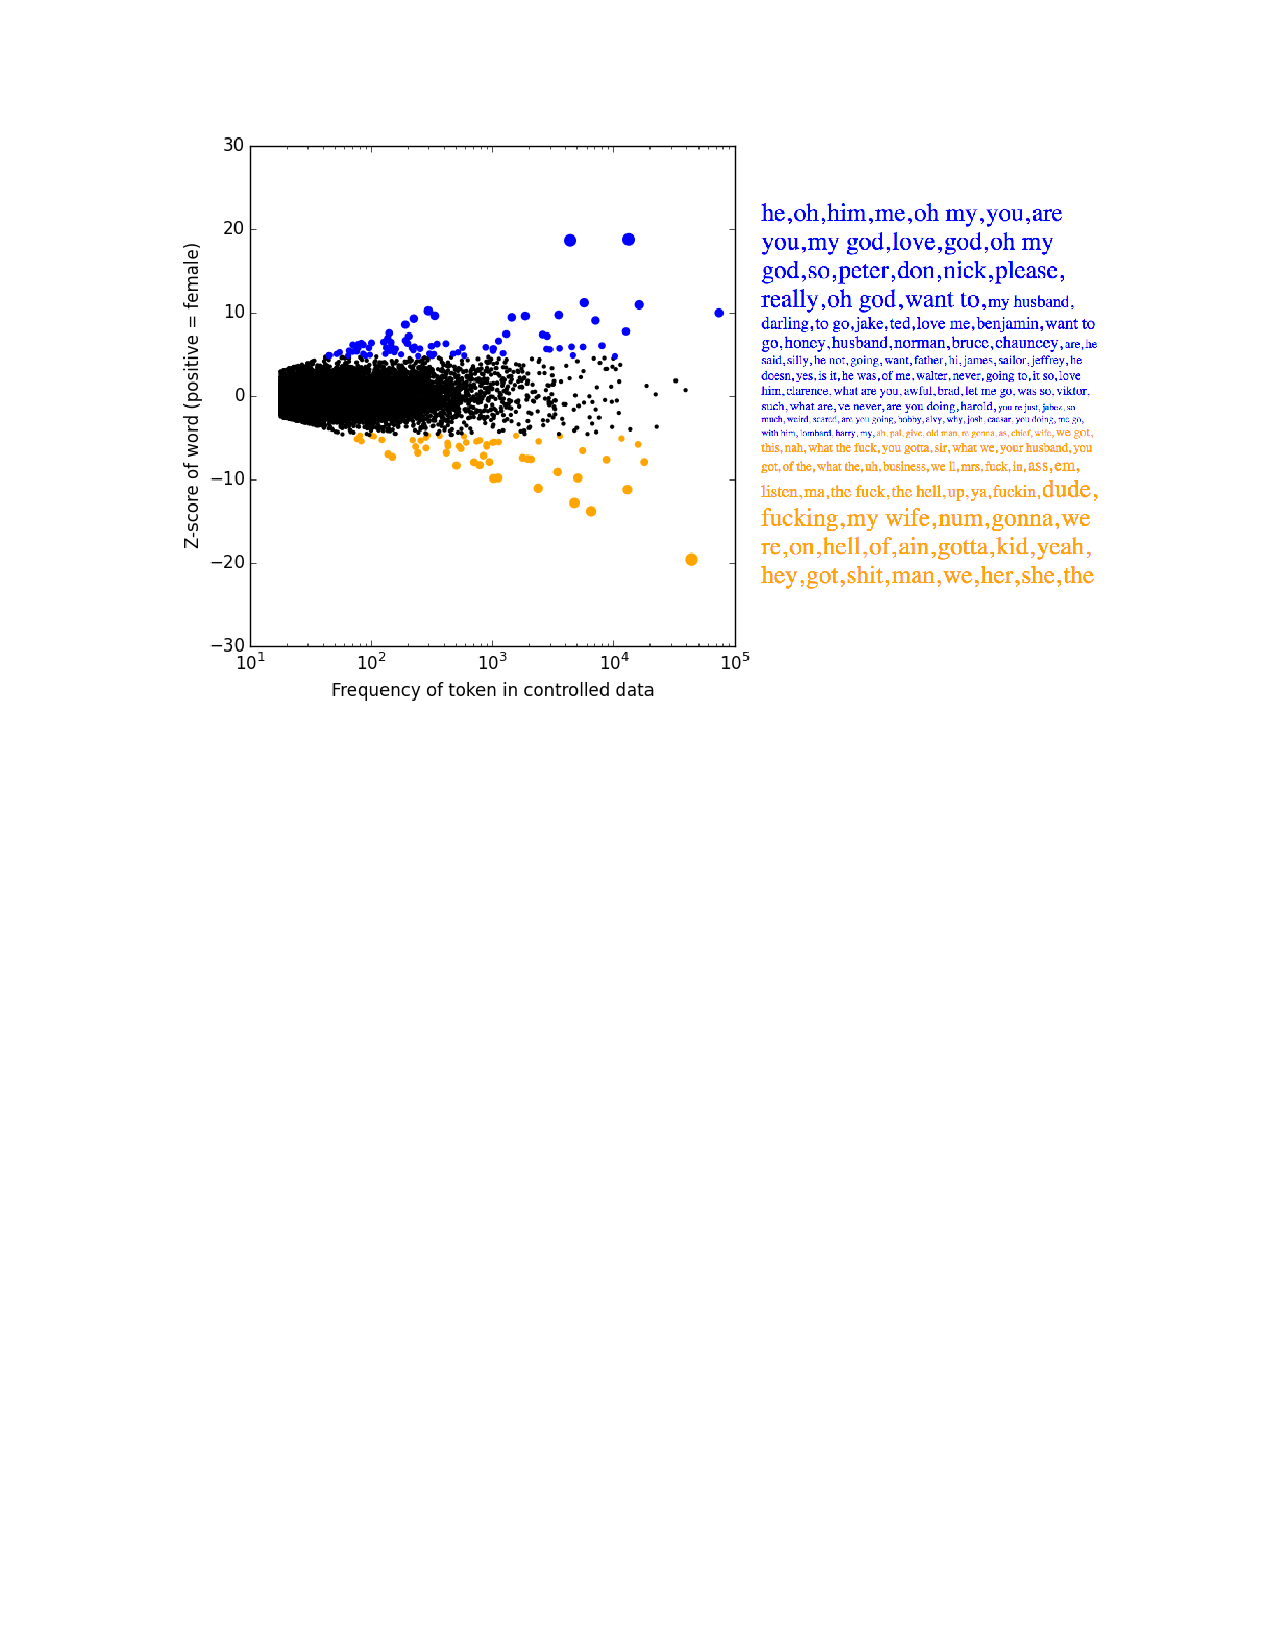
\includegraphics[width=\columnwidth]{Schofield}
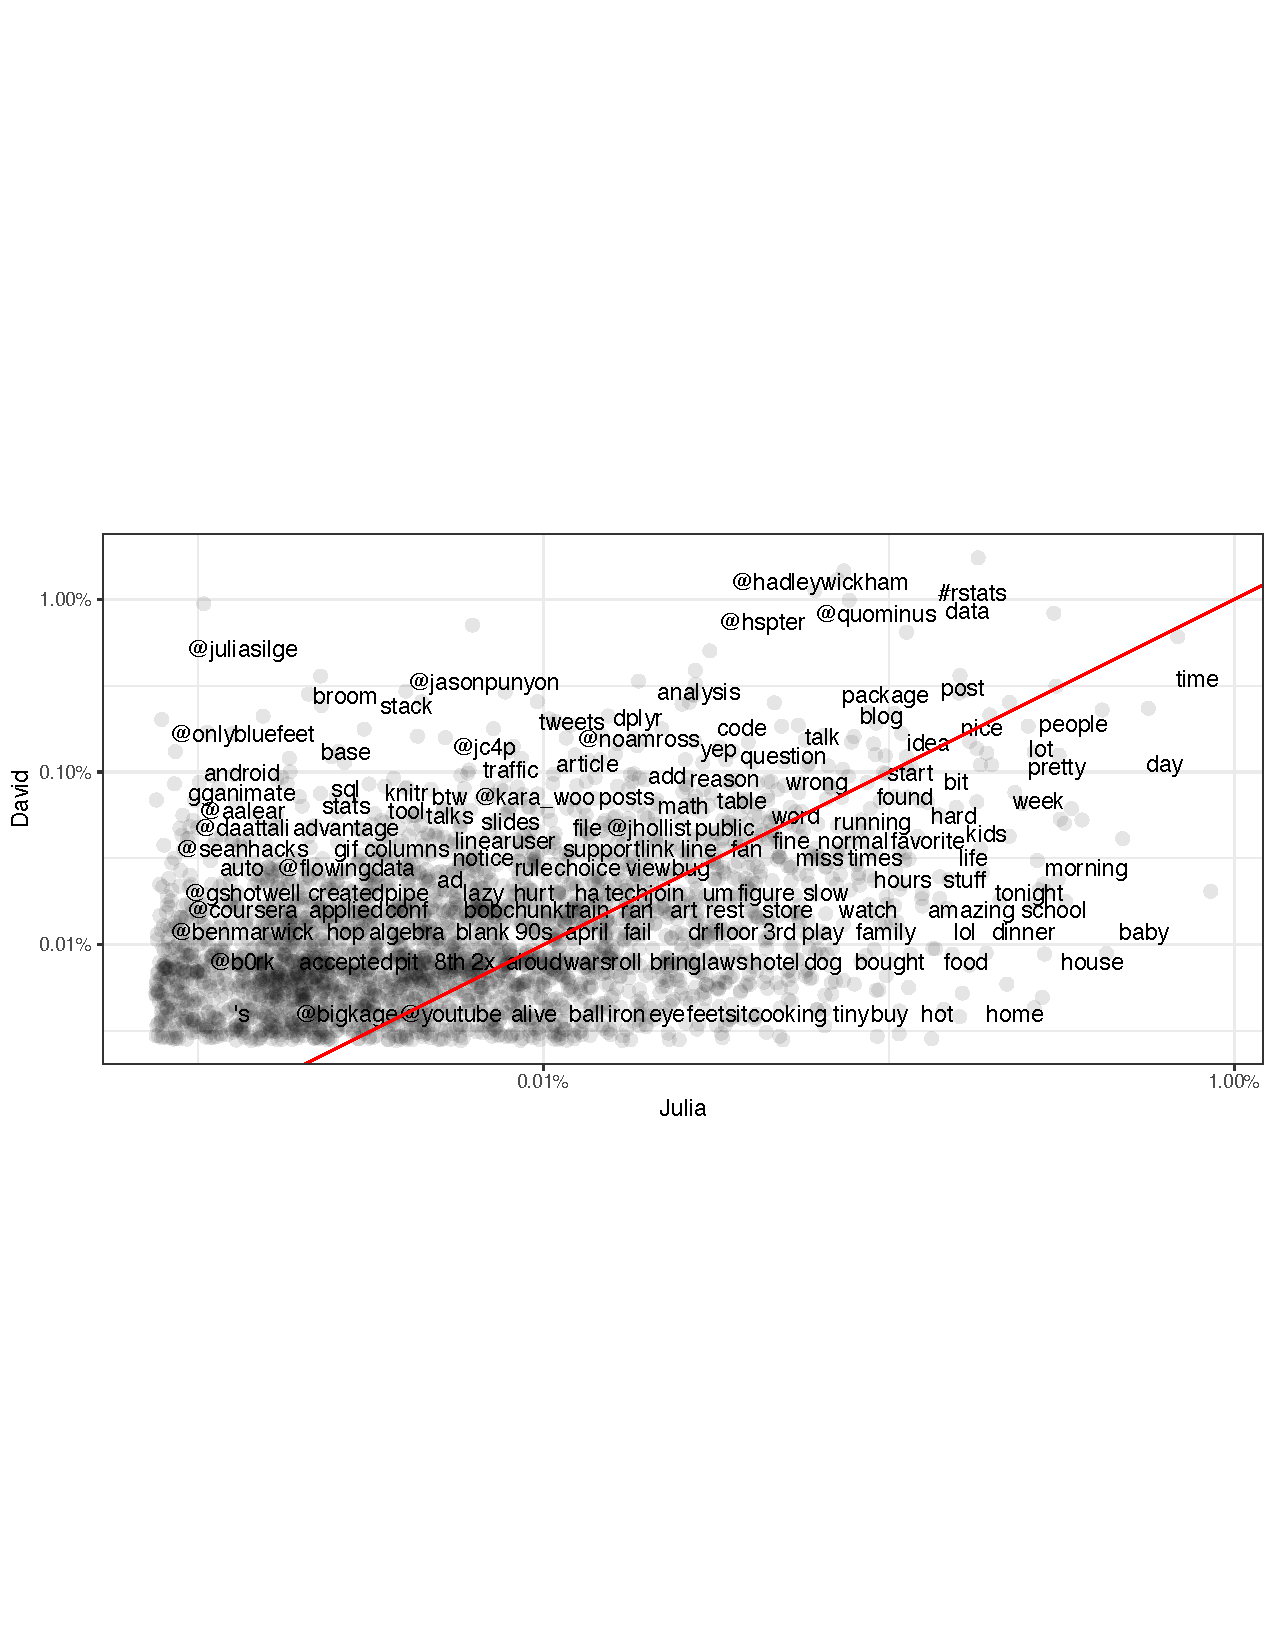
\includegraphics[width=\columnwidth]{tidytext}
\vspace{-1cm}
\caption{Label-overlap solutions are problematic: Schofield and Mehr's (2016) labeling points to the left of the scatter cloud makes relating words and points nearly impossible (top). Tidytext's (Silge and Robinson, 2016) approach involves labeling jittered points using non-overlapping text labels.  Despite the semi-transparency of the points, both labels and points in the interior of the chart are unreadable (bottom).
} 
% Flawed solutions to the label-overlap problem: labeling points to the left of the graph \cite{schofield2016gender} (top) and non-overlapping labels of jittered points \cite{tidytext}.
\vspace{-0.5cm}
\end{figure}

\cite{tidytext}
Labeling points in dense scatter-plots is difficult.  Labels that occur in the 
ggplot2 plots used in tidytext (add citation) often overlap other points, rendering interior labels unreadable. 

Traditionally, points are randomly jittered.  Adding jitter has two disadvantages: 

(1) Some points will randomly appear closer to an upper-left or lower-right-hand corner than others, potentially even those which are more associated with a class, or closer to an axis.  One could address this by coloring points based on their association, but a mix of point colors (show figure) appear can appear disorienting and unaesthetic. 

(2) Jitter makes the point cloud more dense, allowing less space for point labels in the interior of the cloud.  

\section{Scattertext}
\label{scattertext}

Term labeling that prioritizes weights. \cite{cozy}, solves overlapping text and point problem.  When sparse term weights are shown, color zero-points in dark gray, optionally place labels over them.  

interactive-- click to see contexts.  Mousing over points give statistics, and mousing over labels indicates placement of points.  Sidebars of associated and characteristic terms can be moused-over to see placement of term on scatter chart.

Mention size limits, and manual tuning.  

Cross-lingual (e.g., chinese, cite segmenter)

PMI for phrase recognition.

Uses spacy. (cite)

Terms are given category-association scores based on their distance to the upper-left (category \textit{A}) or lower-right (category \textit{B}) corner.

\begin{equation}
  \mbox{insert rudder score here}
  \label{eqn:cornerscore}
\end{equation}

\begin{figure*}[h]
  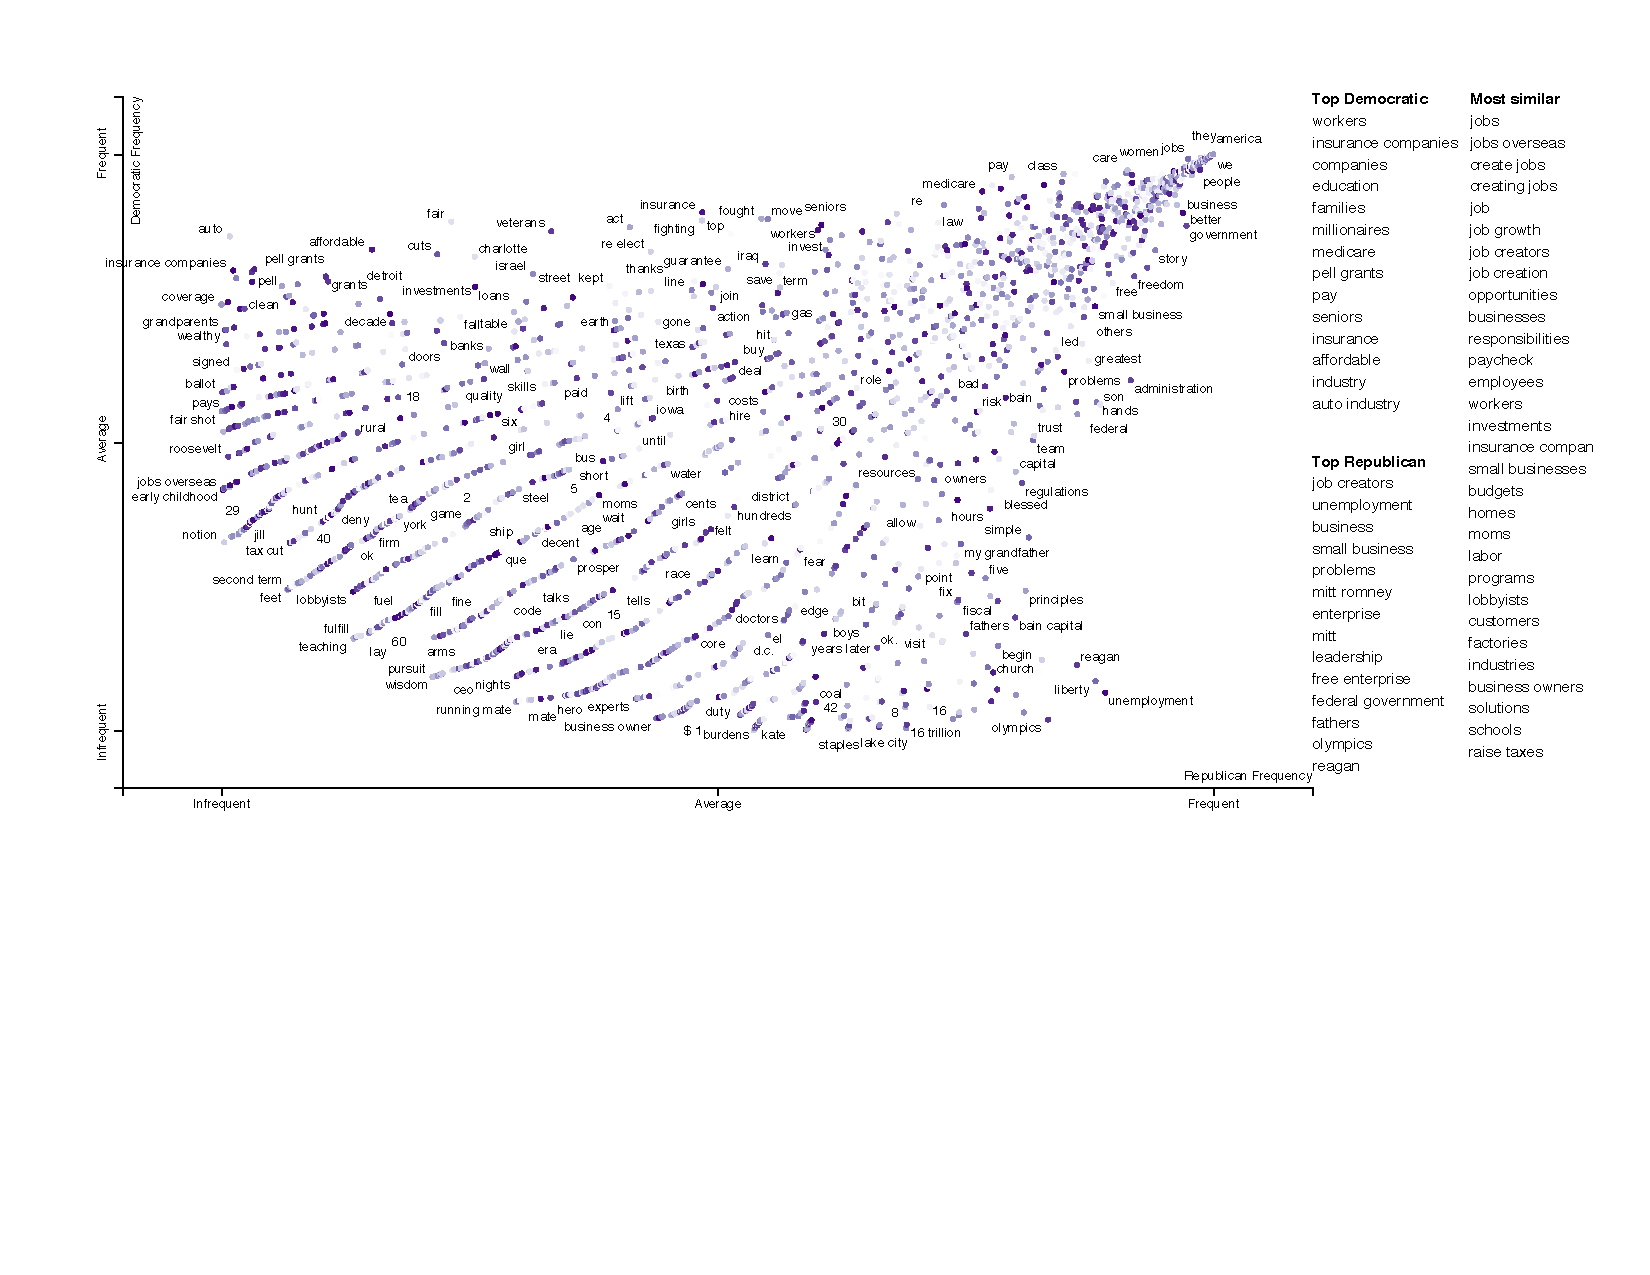
\includegraphics[width=\linewidth]{similarity_scattertext}
  \caption{Words and phrases that are semantically similar to the word ``jobs`` are colored darker, proportional to their cosine similarity over GloVe vectors.}
\end{figure*}


Points are colored based on their based on their highest category-association score.  Points closest to the upper-left-hand corer are colored in progressively darker shades of blue, whiles those closest to the lower-right hand corder in progressively darker shades of red.  To prevent points approximately equidistant from both corners from turning white and blending into the background, they progressively turn yellow.  The colors are provided by D3's ``RdYlBu'' diverging-color scheme. \cite{d3}

Talk about relationship to log-odds.  Points on axes represent infinite log-odds. 

\section{Semantically Similar Category Discriminators}
\label{embeddings}

Suppose you would like to see how see how presidential candidates used language relating to a word like ``job'', ``healthcare'', or ``military'' in presidential debates.  

Using spaCy-provided GloVe \cite{glove} word vectors trained on the Common Crawl corpus (cite glove, spacy), the cosine distance between the target word and each term is computed.  Points on the chart were colored by their similarity to the the target word, but still positioned on the chart based on their category-specific mention-frequency.

In the previous example, identifying the top category-associated terms to display was straight-forward--rank terms based on their euclidean distance to a corner (Equation \ref{eqn:cornerscore}).  This scenario adds the constraint that high scoring terms should be semantically similar to the target term. 

Since the scores are not only on separate scales $[0,1]$ for cosine distance and $[0, \sqrt{2}]$ for euclidean but also differently distributed, the mean of both scores may end up being biased toward one.  To resolve these scaling and distributional differences, both scores transformed using the non-parametric percentile rank transform.  To ensure both scores are relatively high, the harmonic mean is used to combine these transformed scores.


\nocite{ggplot2}
\bibliographystyle{acl}
\bibliography{kessler2017}

\end{document}